\chapter{Estudo de caso}\label{cap:estudos_de_caso}

\begin{citacao}
\traducao{Para fundamentar a discussão em música, considere uma peça de \emph{jazz}, onde \emph{jazz} é um conceito e uma composição particular é uma instância de um conceito. O musicista, explorando os limites do \emph{jazz}, encontra então uma peça para além das regras usuais do \emph{jazz}. Através deste processo, os limites do gênero musica podem ser redefinidos em algum grau, ou se a peça está em um novo terreno particularmente fértil, um novo sub-gênero de \emph{jazz} emerge. Contudo uma peça de música que não quebra limites, de alguma forma pode ser considerada não-criativa.}{
To ground the discussion in music, consider a piece of jazz, where jazz is the concept and the particular composition is an instance of that concept. The musician, in exploring the boundaries of jazz, then finds a piece beyond the usual rules of jazz. Through this process, the boundaries of a music genre may be redefined to some degree, or if the piece is in particularly fertile new ground, a new sub-genre of jazz may emerge.  Indeed a piece of music which does not break boundaries in some way could be considered uncreative.}
\end{citacao}

O objetivo deste capítulo será detalhado na \autoref{sec:objetivo}. Seu contexto inicia com dois registros audiovisuais de \emph{A Study in Keith}, publicados por \citeonline{sorensen_youtube_2014} e \citeonline{sorensen_keith_2009}. São o mesmo registro, mas com duas descrições diversas de um mesmo espaço conceitual \csf{E}{ask}. Existe uma semelhança entre as explicações: um referente opcional \pressingthree{R}{ask}{0} são os Concertos \emph{Sun Bear} \ver{sec:sunbear}. \citeonline{sorensen_youtube_2014} indica outros referentes, \pressingthree{R}{ask}{1} como o ambiente de programação \emph{Impromptu} e \pressingthree{R}{ask}{2} a linguagem de programação \emph{Scheme} \ver{sec:impromptu}: 

\begin{citacao}
\traducao{\emph{A Study in Keith} é uma performance de programação ao vivo por Andrew Sorensen, inspirado nos concertos \emph{Sun Bear} de Keith Jarret. Toda a música que você ouve é gerada a partir do código do programa que é escrito e manipulado em \emph{tempo-real} durante a performance. O trabalho foi executado usando o ambiente de desenvolvimento $[$em linguagem$]$ Scheme $[$chamado$]$ Impromptu (\url{http://impŕomptu.moso.com.au}). Não é Keith, mas inspirado por Keith \cite{sorensen_youtube_2014}.
}
{
``A Study In Keith'' is a live programming performance by Andrew Sorensen inspired by Keith Jarrett's Sun Bear concerts. All of the music you hear is generated from the program code that is written and mani$[$p$]$ulated in real-time during the performance. The work was performed using the Impromptu Scheme software development environment (\url{http://impromptu.moso.com.au}). Not Keith, but inspired by Keith.
}
\end{citacao}

Uma breve análise de uma sonoridade cadencial de um dos concertos será investigada para encontrar outros possíveis referentes opcionais \ver{sec:sunbearanal}. As mensagens codificadas no ambiente \emph{Impromptu} são enviadas para um segundo \emph{software}, um instrumento virtual de estúdio (VSTi), que atua como um simulador de teste para a utilização em um instrumento acústico em uma vinheta nomeada \emph{Disklavier Sessions} \ver{sec:NI}. É indicado também um evento sonoro muito recorrente na improvisação de códigos. O silêncio é, com suas variações temporais, uma constante em outros trabalhos de Sorensen \ver{sec:silencio}:

\begin{citacao}
\traducao{\emph{A Study In Keith} é um trabalho para piano solo (NI's Akoustik Piano), inspirado nos concertos \emph{Sun Bear} de Keith Jarrett. \textbf{Note que não existe som durante os dois primeiros 2 minutos da performance, enquanto estruturas iniciais são construídas}. Não é bem Keith, mas inspirado por Keith \cite{sorensen_keith_2009}}{"A Study In Keith" is a work for solo piano (NI's Akoustik Piano) by Andrew Sorensen inspired by Keith Jarrett's Sun Bear concerts. Note that there is no sound for the first 2 minutes of the performance while initial structures are built. Not quite Keith, but inspired by Keith.}
\end{citacao}


\section{Objetivo}\label{sec:objetivo}

Como pontua \citeonline[p.~121]{McLean2011} \traducao{Nosso estudo de caso é de alguma forma simplista e não é intenção ilustrar uma grande arte ou um grande código. Contudo delineia um processo criativo de classes, como efetuado pelo presente autor.}{Our case study is somewhat simplistic, and is not intended to illustrate either great art or great code. However it does trace a creative process of sorts, as carried out by the present author.}

Este capítulo tratará sobre um grupo finito de blocos de eventos, $[$\pressingthree{E}{ask}{0}$,\ldots,$\pressingthree{E}{ask}{2}$]$, para investigar qual é um primeiro objetivo \pressingtwo{G}{0} \ver{sec:eventos}. Será apresentado também uma classe objetos \pressingtwo{O}{ask} (uma figura de notas) pertinente para entender como este início de improviso inclue uma característica \pressingtwo{F}{ask}{N} semelhante à \emph{Illiac Suite} de \citeonline{hiller_experimental_1959}, mas aplicado ao piano solo. 

\section{Referentes Opcionais}\label{sec:sunbear}

\subsection{Concertos Sun Bear}\label{sec:sunbearanal}

Os concertos \emph{Sun Bear} são originalmente dez LPs  de improvisações de Keith Jarret no Japão, produzidos pela \emph{ECM Records}\footnote{http://www.ecmrecords.com/} entre 1976 e 1978. É o terceiro dos concertos de improvisação que incluem o \emph{Solo Concerts: Bremen/Lausanne} (1973) e \emph{The Köln Concert} (1975).

Foram realizados e gravados como sessões de improvisação contínua, variando entre 31 a 43 minutos cada. Para cada dia, duas sessões de improvisação, em cidades diferentes. Kyoto, 5 de novembro\footnote{Disponível em \url{https://www.youtube.com/watch?v=T2TfIQNxhjc}.}; Osaka, 8 de novembro\disponivelem{https://www.youtube.com/watch?v=FC4iZ1wMoU8}; Nagoya, 12 de novembro\footnote{\url{https://www.youtube.com/watch?v=3a7ezm3D1jA}.}. Tokyo, 14 de novembro\disponivelem{https://www.youtube.com/watch?v=ZH8VIjjhPQ4}; Sapporo, 18 de Novembro\disponivelem{https://www.youtube.com/watch?v=BqYBT_HoG4M}.


Um documento crítico impresso é mencionado na \emph{internet} como um antigo documento contendo notas discográficas \cite{rollingstone1985}. Seu acesso foi restrito durante a pesquisa, e não foi possível incluir alguma citação. Da mesma forma, documentos análiticos sobre a peça não foram encontrados em alguma base de dados. Existem algumas notas discográficas compiladas por uma comunidade de fãs e críticos musicais estadounidenses. Duas notas sugerem uma descrição da forma musical aplicada por Keith Jarret: \traducao{O tema de \emph{Kyoto Parte 1} é repetido por Keith Jarret no fim de \emph{Kyoto Parte 2}. Então podemos considerar o todo deste concerto como uma grande Suíte.}{The theme of Kyoto Part 1 is repeated By Kj at the end of Kyoto Part 2. So we can consider the whole of this concert as one big Suite}\cite[p.~129]{jarret_discography_2014}. 

\traduzcitacao{Revisto por Richard S. Ginnel\footnote{Disponível em \url{http://www.mcana.org/formembersatlarge.html}.}: $[$--$]$ Este pacote gigantesco -- um conjunto de dez LPs agora comprimidos em uma caixa robusta de seis $[$embalagens de$]$ CDs -- foi ridicularizado uma vez como uma última viagem de ego, provavelmente por muitos que não tomaram um tempo para ouvir tudo. (\ldots) Ainda assim, o milagre é como esta caixa é consistentemente muito boa. \textbf{Na abertura de Kyoto, a meditação direcionada para o \emph{gospel}} está em plena atuação, ao nível de suas melhores performances solo em Bremen e Koln,\textbf{e os concertos Osaka e Nagoya possuem citações de primeira linha, geralmente do tipo \emph{folk}}, mesmo profundas, idéias líricas
}{
Review by Richard S. Ginell: $[$--$]$ This gargantuan package -- a ten-LP set now compressed into a chunky six-CD box -- once was derided as the ultimate ego trip, probably by many who didn't take the time to hear it all. You have to go back to Art Tatum's solo records for Norman Granz in the '50s to find another large single outpouring of solo jazz piano like this, all of it improvised on the wing before five Japanese audiences in Kyoto, Osaka, Nagoya, Tokyo, and Sapporo. Yet the miracle is how consistently good much of this giant box is.  In the opening Kyoto concert, Jarrett's gospel-driven muse is in full play, up to the level of his peak solo performances in Bremen and Koln, and the Osaka and Nagoya concerts have pockets of first-rate, often folk-like, even profound, lyrical ideas.
}
{p.~130}
{jarret_discography_2014}

O \emph{gospel} e o \emph{folk} são citados como gêneros musicais inclusivos nesta suíte. Porém esta Suíte não possui pausas entre as partes (o improviso é contínuo, mas seccionado por transições). Uma transcrição do motivo gerador deste \emph{gospel} no concerto de Kyoto buscou encontrar referentes opcionais adicionais para \pressingtwo{R}{ask} (isto é, informações de harmonia e ritmo), mesmo com a afirmação anterior que nenhuma relação pode ser encontrada \ver{fig:Jarret_intro}. 

\begin{figure}[!h]
  \centering
  %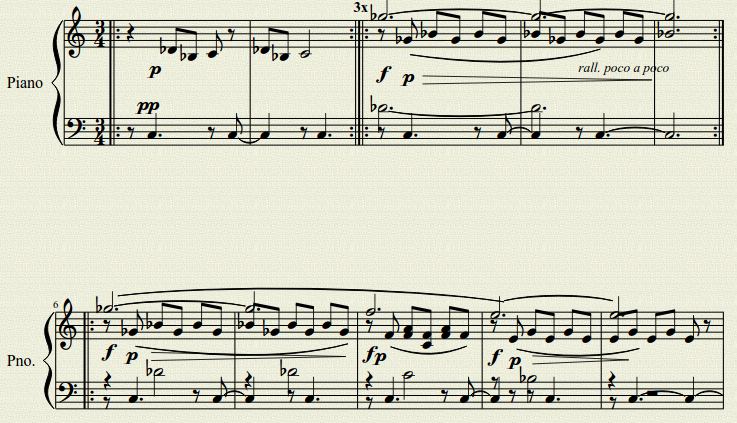
\includegraphics[scale=0.5]{imagens/Jarret_intro.png}
  {%
\parindent 0pt
\noindent
\ifx\preLilyPondExample \undefined
\else
  \expandafter\preLilyPondExample
\fi
\def\lilypondbook{}%
\input{b1/lily-fc418522-systems.tex}
\ifx\postLilyPondExample \undefined
\else
  \expandafter\postLilyPondExample
\fi
}
  \caption{Transcrição do motivo gerador do disco Kyoto, parte 1. \textbf{Fonte}: autor.}
  \label{fig:Jarret_intro}
\end{figure}


O bloco de sonoridades iniciais \pressingthree{E}{ask}{0} sugere alguma referência à forma Fantasia Cromática ou um Prelúdio, no sentido de um jogo livre que prepara o improvisador para a sonoridade do instrumento no ambiente tocado.  Uma sonoridade oscilante é colocada em movimento num âmbito de terça menor nos compassos 1 e 2 entre Si bemol, Dó e Ré Bemol, repetindo 3 vezes (\pressingthree{P}{KJ}{0}) dois objetos \pressingthree{O}{KJ}{0} e \pressingthree{O}{KJ}{1}: um ostinato na mão esquerda e uma bordadura na mão direita . Nos compassos 3 a 5 um terceiro objeto \pressingthree{O}{KJ}{2}, um acorde de Sol bemol Maior (transcrito assim para facilitar a leitura), dividido em uma quarta justa entre a mão esquerda e direita, com terças alternadas em colheias na mão direita. Este evento é então expandido nos compassos 6 a 10, gerando uma figura cromática proto-melódica, cujo acompanhamento harmônico segue, curiosamente, uma progressão de substituição por trítono (este motivo está sendo considerando como parte do  \emph{gospel} supracitado): Sol Bemol Maior, Fá Maior com sexta adicionada (ou Ré menor com sétima) e Dó Maior com sétima menor. Inicialmente, consideramos esta progressão do ponto de vista de \citeonline[p.~27]{soares_luteria_2015}, Fá sustenido Maior pode ser descrito como um \emph{contra-polo} de Dó (ver \autoref{fig:eixo}). Porém Dó realiza no final deste bloco uma função de dominante (V$^7$), o que sugere que o acorde anterior é umauma subdominante relativa com a sétima no baixo ($_7$II). Uma possibilidade neste tipo de análise, mais próxima da visão do \emph{jazz}, seria indicar o Fá sustenido como uma $_b$V/V (subV), sem a sétima e acompanhado de uma nota pedal. 

\begin{figure}[!h]
  \centering
  \includegraphics[scale=0.4]{/home/guilherme/Github/luteria/axis/PoloContrapolo.png}
  \caption{Sistema de Eixos - Rotacão entre primário e secundário. \textbf{Fonte}: \citeonline{soares_luteria_2015}}
  \label{fig:eixo}
\end{figure}

\subsection{NI-Akoustik Piano}\label{sec:NI}

O NI, é uma abreviação para \emph{Native Instruments}, uma empresa de tecnologias para áudio \footnote{Disponível em \url{http://www.native-instruments.com/en/company/}.}. O \emph{Akoustic Piano} é uma extensão (\emph{plugin}) VST, que emula diferentes pianos acústicos. Entre os instrumentos utilizados, incluem o \emph{Bösendorfer 290 Imperial}, \emph{Steinway D}, e \emph{Bechstein D 280}\footnote{Disponível em \url{http://www.kvraudio.com/product/akoustik-piano-by-native-instruments}.}. Os instrumentos são gravados nota a nota por um complexo sistema de tomada de som. Na \autoref{fig:NI}, a gravação de um outro VSTi ilustra como é realizado o processo (no caso, por Uli Baronowsky)

\begin{figure}[!h]
  \centering
  %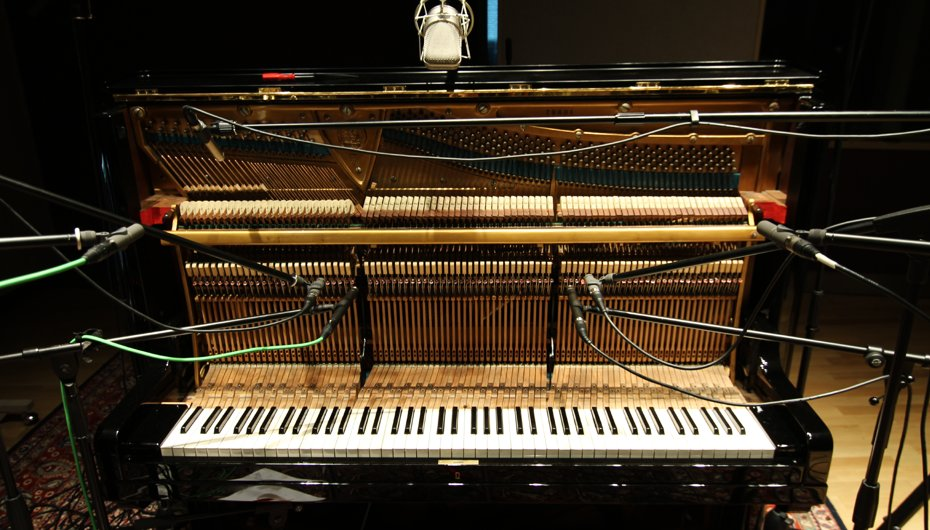
\includegraphics[scale=0.4]{imagens/piano.png}
  \caption{Sistema de tomada de som para produção de um VSTi. \textbf{Fonte}: \url{http://www.native-instruments.com/en/products/komplete/keys/definitive-piano-collection/}}
  \label{fig:NI}
\end{figure}

ou em um instrumento acústico modificado, como o \emph{Disklavier} da Yamaha \ver{fig:disklavier}. Este último caso não é citado por \citeonline{sorensen_youtube_2014} e \citeonline{sorensen_keith_2009}, masem \emph{Disklavier Sessions} \cite{sorensen_disklavier_2013} é semelhante à atividade descrita em \emph{A Study in Keith}:

\begin{figure}[h]
  \centering
  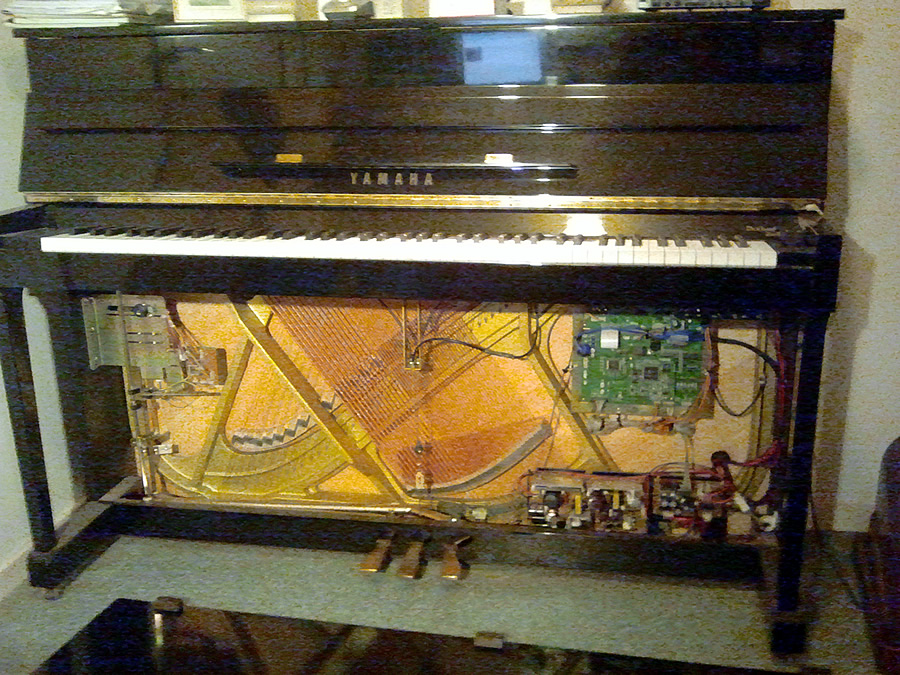
\includegraphics[scale=0.5]{imagens/disklavier.jpg}
  \caption{Piano Disklavier de armário, com a parte interna exposta para exibir a placa-mãe. \textbf{Fonte}: wikimedia.org}
  \label{fig:disklavier}
\end{figure}

\begin{citacao}
\traducao{Em \emph{Disklavier Sessions} os programas escritos em tempo-real por Ben e Andrew geram um fluxo de dados de notas que são enviados para ser executado em um piano disklavier mecanizado. Assim como as alturas das notas, toda a performance do piano deve ser codificada na informação gerada pelo programa e enviada para o piano disklavier.}{In the Disklavier Sessions the programs beign written in real-time by Ben and Andrew are generating a live stream of note data which is sent to a mechanized disklavier piano to be performed. As well the individual note pitches all of the piano performance must be encoded into the information being generated by the program and sent to disklavier piano}
\end{citacao}


\subsection{Ambiente e Linguagem: Impromptu}\label{sec:impromptu}

\begin{citacao}
\traducao{
Impromptu é uma linguagem e um ambiente de programação OSX\footnote{Sistema Operacional Mac OSX.} para compositores, artistas sonoros, VJ's e artistas gráficos  com um interesse em programação ao vivo ou interativa. Impromptu  é um ambiente de linguagem Scheme, um membro da família das linguages Lisp. Impromptu é usado por artistas-programadores em performances de \emph{livecoding} em torno do mundo.
}{
Impromptu is an OSX programming language and environment for composers, sound artists, VJ's and graphic artists with an interest in live or interactive programming. Impromptu is a Scheme language environment, a member of the Lisp family of languages. Impromptu is used by artist-programmers in livecoding performances around the globe.
}
\end{citacao}

Existe uma restrição quanto ao nicho de usuários do \emph{software}. É indicado que este grupo é restrito aos usuários de computadores Apple; no entanto uma investigação indica que o código-base é desenvolvido em um nível acima de outro, \emph{Extempore}.

\citeonline[p. 823] {sorensen_impromptu_2010} que o \emph{ambiente de programação ciberfísico} é análogo à \emph{partitura} tradicional; sua diferença está ligada à sua execução imediata. Nos termos de \citeonline{mathews_groove_1970}, uma \emph{engenharia humana}. Nos termos de \citeonline[p.~5]{fenerich_marulho_2014}, uma programação-partitura:

\begin{citacao}
\traducao{Considere a analogia da partitura musical tradicional. A partitura provê uma especificação estática da intenção -- um programa de domínio estático. Musicistas, representam o domínio do processo, executam ações requeridas para realizar ouo reificar a partitura. Finalmente, as ações no domínio do processo resultam em ondas sonoroas que são percebidas por uma audiência humana como música. Este estágio final é o nosso domínio real de trabalho. Agora considere um domínio de programação dinâmica no qual o compositor concebe e descreve uma partitura em \emph{tempo-real}. Nós geralmente chamamos este tipo de composição de improvisação. \textbf{Na improvisação o(a) musicista é envolvido em um circuito-fechado retroalimentado que envolve premeditação, movendo para ação casual e finalmente para reação, refinamento e reflexão.}}{
Consider the analogy of a traditional musical score. The score provides a static specification of intention – a static program domain. Musicians, representing the process domain, perform the actions required to realise or reify the score. Finally, the actions in the process domain result in sound waves which are perceived by a human audience as music. This final stage is our real-world task domain. Now consider a dynamic program domain in which a composer conceives of and describes a musical score in real-time. We commonly call this type of composition improvisation. In it, the improvising musician is involved in a feedback loop involving
forethought, moving to causal action and finally toreaction, refinement and reflection.}
\end{citacao}

\subsection{Extempore}

O \emph{Extempore} possui uma filosofia próxima àquela descrita por \citeonline{mathews_groove_1970}, isto é, de um sistema humano-máquina reflexivo. Um nome específico é dado para a atividade de escrita do código, ou \emph{programação ciberfísica}:

\begin{citacao}
\traducao{\emph{Extempore} é projetado para suportar um estilo de programação apelidado de $[$''$]$programação ciberfísica''.Programação ciberfísica suporta a noção de um programador humano operando como um agente ativo em uma rede de \emph{tempo-real} distribuída de sistemas ambientalmente conscientes} {Extempore is designed to support a style of programming dubbed 'cyberphysical' programming. Cyberphysical programming supports the notion of a human programmer operating as an active agent in a real-time distributed network of environmentally aware systems. \disponivelem{https://github.com/digego/extempore}. }
\end{citacao}

Entre suas características incluem\disponivelem{http://benswift.me/2012/08/07/extempore-philosophy/}:

- Processamento de Sinais Digitais (DSP) \footnote{Sobre DSP, \cfcite{smith_dsp_2012}.} em  tempo-real;

- Sequenciamento de áudio (baseado em notas) de alto-nível\footnote{Como o disparo de sons baseado em parâmetros como altura, intensidade e duração. Disponível em \url{http://benswift.me/2012/10/15/playing-an-instrument-part-i/}.};

- Processamento de gráficos;


A segunda característica será explorada neste capítulo como base técnica para o processo criativo em \emph{Study in Keith}

\subsection{Scheme}\label{sec:scheme}

Scheme (1970) é citado na \emph{internet} como uma definição de linguagem, ou dialeto, da linguagem Lisp (1958). Como uma linguagem imperativa orientada à expressões, utiliza \emph{representações simbólicas} de listas, para definir rotinas que podem definir outras rotinas. Esta característica habilitou programadores a realizarem uma atividade conhecida como \emph{meta-programação}.

\begin{example}{Notação Scheme}
Neste tipo de notação (\emph{prefix notation}, ou notação prefixada), são listados \emph{átomos}, que podem ser números, operadores, funções ou outras listas. Por exemplo. Uma divisão de dois números, pode ser escrita de maneira bastante simples:

\begin{minted}{cl}
;; uma operacao de divisao
(/ 1 2)

;; pode ser mais descritiva
(define divide (lambda (a b) (/ a b)))

;; execucao
(divide 1 2)
\end{minted}
\end{example}

Um exemplo musical é sugerido por \citeonline[p.~823-824]{sorensen_impromptu_2010} como fonte para um pseudo-código documentado. É possível notar uma ênfase em um discurso camerístico, na improvisação com instrumentos acústicos e sons eletrônicos, e uma base harmônica tonal comum:

\begin{example}{Exemplo imaginário}

NOTA: o processo será realizado de maneira semelhante àquele descrito por \citeonline{mathews_groove_1970} (\autoref{sec:groove}, p.~\pageref{sec:groove}), isto é, a partir de um circuito-fechado entre executante, máquina e projetores (visuais e acústicos).

\begin{citacao}
\traducao{
\small{Dois performers se apresentam no palco. Um violinista, em pé e parado, com seu arco preparado. Outro senta-se atrás do brilho da tela do \emph{laptop}. Uma projeção da tela do \emph{laptop} é projetada acima do palco, e mostra uma página em branco, com um simples cursor piscando. O musicista-programador começa a digitar \ldots}
}{
Two performers are present on stage. One, a violinist, stands paused, bow at the ready. Another sits behind the glow of a laptop screen. A projection of the laptop screen is cast above the stage showing a blank page with a single blinking cursor. The laptop musician begins to type ...
}
\end{citacao}

\begin{minted}{cl}
( play-sound ( now ) synth c3 soft minute)
\end{minted}

\begin{citacao}
\traducao{
\small{\ldots a expressao é avaliada, e lampeja no retroprojetor para exibir a ação do executante. Um som etéreo sintetizado entra imediatamente no espaço e o violinista começa a improvisar em simpatia com a novidade da textura. O músico-programador, ouve o material temático fornecido pelo violinista e começa a delinear um processo generativo Markoviano para acompanhar o violino:}
}
{
\ldots the expression is evaluated and blinks on the overhead projection to display the performer’s action. An ethereal synthetic sound immediately enters the space and the violinist begins to improvise in sympathy with the newly evolving synthetic texture. The laptop performer, listens to the thematic material provided by the violinist and begins to outline a generative Markov process to accompany the violin ...
}
\end{citacao}

\begin{minted}{cl}
( define chords
  ( lambda ( beat chord duration )
    ( for-each ( lambda ( pitch )
                   ( play synthj pitch soft duration ))
               chord )
    ( schedule (* metro * ( + beat duration )) chords
               (+ beat duration )
               ( random ( assoc chord (( Cmin7 Dmin7 )
                                       ( Dmin7 Cmin7 ))))
               duration )))

( chords (* metro * get-beat 4) Cmin7 4)
\end{minted}

\begin{citacao}
\traducao{\small{\ldots A função \emph{chords} é chamada no primeiro tempo de um novo xxxxxxx e uma simples progressão recursiva de acordes come a suportar a performance melódica do violino. A função \emph{chords} cria um laço temporal, gerando uma sequência interminável de acordes de quatro tempos. Depois de poucos momentos de reflexão, o musicista-programador começa a modificar a função \emph{chords} para suportar uma progressão de acordes mais variada, com uma razão aleatória $[$em função$]$ da recursão temporal\ldots}}
{\ldots the “chords” function is called on the first beat of a new common time bar and a simple recursive chord progression begins supporting the melodic performance of the violin. The chord function loops through time, creating an endless generative sequence of four beat chords. After a few moments of reflection the laptop performer begins to modify the “chords” function to support a more varied chord progression with a randomised rate of temporal recursion\ldots}
\end{citacao}

\begin{minted}{cl}
( define chords
  ( lambda ( beat chord duration )
    ( for-each ( lambda ( pitch )
                   ( play dls (+ 60 pitch) soft duration ))
               chord )
    ( schedule (* metro * ( + beat duration )) chords
               (+ beat duration )
               ( random ( assoc chord (( Cmin7 Dmin7 Bbmaj )
                                       ( Bbmaj Cmin7 )
                                       ( Dmin7 Cmin7 )))
               ( random (3 6))))))

( chords (* metro * get-beat 4) Cmin7 4)
\end{minted}
\end{example}

\section{Blocos de Eventos}\label{sec:eventos}

\subsection{Primeiro evento sonoro: a sensação de quietude}\label{sec:silencio}

Uma nota pertinente sobre esta improvisação feita pelo próprio Sorensen: nos primeiros dois minutos do vídeo (aproximadamente 1$'$53$''$). existe um silêncio. Este silêncio é característico daquele momento em que os primeiros códigos são escritos.

Este comportamento, do tempo de codificação, ao tempo de ação musical, é similar em outros dois vídeos, de Sorensen: \sorensen{An evening of livecoding at 53 Rusden Street}{https://vimeo.com/2433303}, \sorensen{Just for Fun}{https://vimeo.com/2433971}, \sorensen{A Study in Part}{https://vimeo.com/2434054}, \sorensen{Stained}{https://vimeo.com/2502546}, \sorensen{Transmissions in Sound}{Transmissions in Sound}, \sorensen{Antiphony}{https://vimeo.com/2503188},  \sorensen{Strange Places}{https://vimeo.com/2503257}, \sorensen{Orchestral}{https://vimeo.com/2579694}, \sorensen{UMDT}{https://vimeo.com/2579880}, \sorensen{Day of Triffords}{https://vimeo.com/2735394}, \sorensen{Face to Face}{https://vimeo.com/5690854}, \sorensen{BM\&E}{https://vimeo.com/7339135}, \sorensen{A Christimas Carol}{https://vimeo.com/8364077} \sorensen{Dancing Phalanges}{https://vimeo.com/8732631}, \sorensen{Livecoding Audio DSP}{https://vimeo.com/15585520}, \sorensen{Jazz Ensenble Study}{https://vimeo.com/15679078}, \sorensen{Variations on a Christmas Theme}{https://vimeo.com/18008372}.

Seu início é um pequeno comentário que contêm o nome do executante e seu email para contato (primeiros sete segundos), bem como a escrita de um código que inicializa o NI-Akoustik (até 0$'$43$''$, ver \autoref{fig:SIK_piano}). 

\begin{figure}[!h]
  \centering
  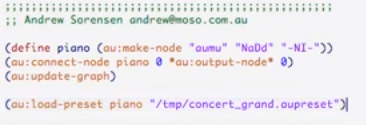
\includegraphics[scale=0.7]{imagens/SIK_piano.png}
  \caption{Primeiros eventos musicais gerados a partir das primeiras estruturas válidas de código. \textbf{Fonte}: autor.}
  \label{fig:SIK_piano}
\end{figure}

Em 0$'$52$''$, Sorensen define um tempo base (ver \autoref{fig:SIK_metro}):

\begin{figure}[!h]
  \centering
  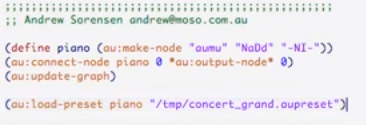
\includegraphics[scale=0.7]{imagens/SIK_metro.png}
  \caption{Definição do tempo base. \textbf{Fonte}: autor.}
  \label{fig:SIK_metro}
\end{figure}

Até 1$'$07$''$, uma rotina que executa acordes é escrita (ver \autoref{fig:SIK_acorde}). É interessante notar que a função \emph{chords} ainda não foi definida.

\begin{figure}[!h]
  \centering
  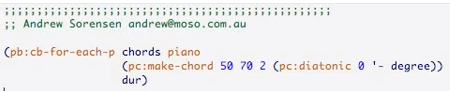
\includegraphics[scale=0.7]{imagens/SIK_chord.png}
  \caption{Criação da rotina que irá executar acordes. \textbf{Fonte}: autor.}
  \label{fig:SIK_acorde}
\end{figure}

Em 1$'$53$''$ a função \emph{chords} é definida de maneira válida, e os primeiros eventos sonoros são criados (ver \autoref{fig:SIK_acorde2}):

\begin{figure}[!h]
  \centering
  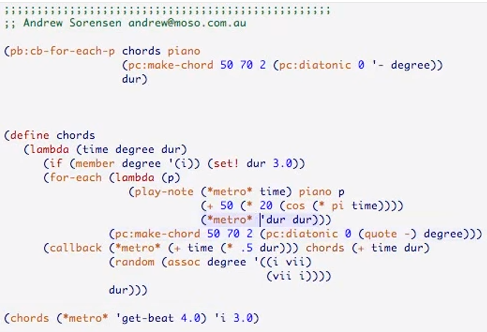
\includegraphics[scale=0.7]{imagens/SIK_chord2.png}
  \caption{Definição da função \emph{chord}. \textbf{Fonte}: autor.}
  \label{fig:SIK_acorde2}
\end{figure}

O restante da improvisação será conduzida a partir da modificação desta função, que a cada tempo, executa um conjunto de notas (inicialmente blocos musicais, que desenvolve para contrapontos floridos, ostinatos e gestos  arpejo/escala), conforme é indicado pelo programador.


\subsection{Segundo Evento Sonoro}\label{sec:segundoevento}

Uma escuta investigativa desta performance considerou o resultado sonoro gerador como replicante de uma escrita contrapontística modal, não-estrita, inicialmente à duas vozes em primeira espécie, que lembra um canto religioso.

Sorensen define um tempo regular de 110 BPM durante o momento de silêncio Os primeiros eventos sonoros que ocorrem após o momento de silêncio foram transcritos considerando a percepção dos tempos fortes e fracos. Isto é, enquanto Sorensen define um tempo regular de 110 BPM, o processo de transcrição
de maneira aproximada em um tempo regular de aproximadamente 40 BPM. A partir disso, cada compasso desta transcrição são dois compassos do vídeo. Segundo o próprio vídeo, o tempo é definido por 110 BPM e cada nota inicial é de quatro tempos, mas que irá sofrer alterações. 

A \autoref{fig:SIK_acorde2} indica que um jogo entre primeiro grau menor, e sétimo grau diminuto será conduzido  (ver \autoref{fig:SIKinicio}).

\begin{figure}[!h]
  \centering
  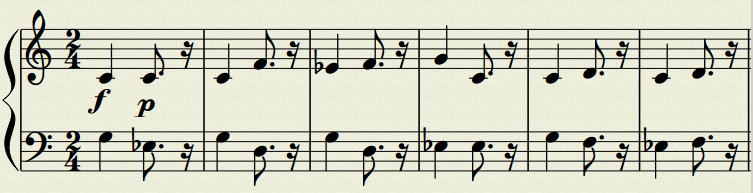
\includegraphics[scale=0.5]{imagens/SIK_motivo.png}
  \caption{Primeiros eventos musicais gerados a partir das primeiras estruturas válidas de código. \textbf{Fonte}: autor.}
  \label{fig:SIKinicio}
\end{figure}

Uma pequena transcrição de uma primeira seção da improvisação é apresentada na \autoref{app:studyinkeith}: uma primeira seção da peça, que vai do 1$'$53$''$ até 4$'$55$''$, pode ser descrita como: um contraponto, inicialmente à duas vozes em primeira espécie (dó eólio), que sofre perturbações sistêmicas. Tais perturbações parecem ser derivadas das intervenções de Sorensen no código do programa.

Tais perturbações criam variações na acentuação, bem como adicionam novas figuras de ritmo, de maneira bastante gradual (ver \autoref{fig:perturba}).

\begin{figure}[!h]
  \centering
  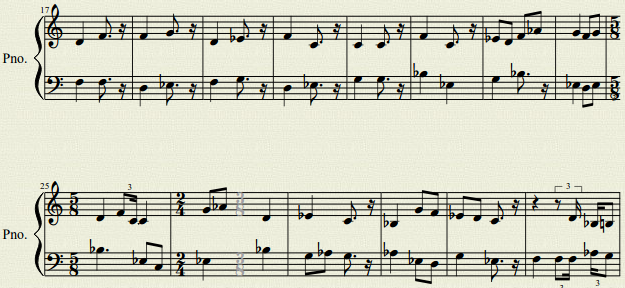
\includegraphics[scale=0.5]{imagens/SIK_perturba.png}
  \caption{Primeiros perturbações sistêmicas. \textbf{Fonte}: autor.}
  \label{fig:SIKinicio}
\end{figure}

No ponto culminante da peça podemos escutar um contraponto florido, adicionado de um ostinato com uma única nota, e algumas intervenções de gestos, arpejos ou escalas em alta velocidade.

Ao final, este conjunto de eventos sonoros

Este conceito nos pareceu bastante similar àquele apresentado por \citeonline{hiller_experimental_1959}. HillerDurante um breve período, algumas regras de contraponto não mantidas;

\subsection{Terceiro Evento Sonoro}\label{sec:terceiro evento}